\documentclass[a4paper,11pt]{article}
\usepackage{amsmath,amsthm,amsfonts,amssymb,amscd,amstext,vmargin,graphics,graphicx,tabularx,multicol} 
\usepackage[francais]{babel}
\usepackage[utf8]{inputenc}  
\usepackage[T1]{fontenc} 
\usepackage{pstricks-add,tikz,tkz-tab,variations}
\usepackage[autolanguage,np]{numprint} 
\usepackage{calc}

\setmarginsrb{1.5cm}{0.5cm}{1cm}{0.5cm}{0cm}{0cm}{0cm}{0cm} %Gauche, haut, droite, haut
\newcounter{numexo}
\newcommand{\exo}[1]{\stepcounter{numexo}\noindent{\bf Exercice~\thenumexo} : }
\reversemarginpar

\newcommand{\bmul}[1]{\begin{multicols}{#1}}
\newcommand{\emul}{\end{multicols}}

\newcounter{enumtabi}
\newcounter{enumtaba}
\newcommand{\q}{\stepcounter{enumtabi} \theenumtabi.  }
\newcommand{\qa}{\stepcounter{enumtaba} (\alph{enumtaba}) }
\newcommand{\initq}{\setcounter{enumtabi}{0}}
\newcommand{\initqa}{\setcounter{enumtaba}{0}}

\newcommand{\be}{\begin{enumerate}}
\newcommand{\ee}{\end{enumerate}}
\newcommand{\bi}{\begin{itemize}}
\newcommand{\ei}{\end{itemize}}
\newcommand{\bp}{\begin{pspicture*}}
\newcommand{\ep}{\end{pspicture*}}
\newcommand{\bt}{\begin{tabular}}
\newcommand{\et}{\end{tabular}}
\renewcommand{\tabularxcolumn}[1]{>{\centering}m{#1}} %(colonne m{} centrée, au lieu de p par défault) 
\newcommand{\tnl}{\tabularnewline}

\newcommand{\trait}{\noindent \rule{\linewidth}{0.2mm}}
\newcommand{\hs}[1]{\hspace{#1}}
\newcommand{\vs}[1]{\vspace{#1}}

\newcommand{\N}{\mathbb{N}}
\newcommand{\Z}{\mathbb{Z}}
\newcommand{\R}{\mathbb{R}}
\newcommand{\C}{\mathbb{C}}
\newcommand{\Dcal}{\mathcal{D}}
\newcommand{\Ccal}{\mathcal{C}}
\newcommand{\mc}{\mathcal}

\newcommand{\vect}[1]{\overrightarrow{#1}}
\newcommand{\ds}{\displaystyle}
\newcommand{\eq}{\quad \Leftrightarrow \quad}
\newcommand{\vecti}{\vec{\imath}}
\newcommand{\vectj}{\vec{\jmath}}
\newcommand{\Oij}{(O;\vec{\imath}, \vec{\jmath})}
\newcommand{\OIJ}{(O;I,J)}


\newcommand{\reponse}[1][1]{%
\multido{}{#1}{\makebox[\linewidth]{\rule[0pt]{0pt}{20pt}\dotfill}
}}

\newcommand{\titre}[5] 
% #1: titre #2: haut gauche #3: bas gauche #4: haut droite #5: bas droite
{
\noindent #2 \hfill #4 \\
#3 \hfill #5

\vspace{-1.6cm}

\begin{center}\rule{6cm}{0.5mm}\end{center}
\vspace{0.2cm}
\begin{center}{\large{\textbf{#1}}}\end{center}
\begin{center}\rule{6cm}{0.5mm}\end{center}
}



\begin{document}
\pagestyle{empty}
\titre{Séance d'AP 2 : Démonstration du théorème de Pythagore}{}{}{4ème}{}

\vspace*{0.2cm}



\underline{Consignes :}\\

- On découpe (deux fois) quatre triangles dans deux rectangles de même dimension a et b, de diagonale c.



\begin{center}
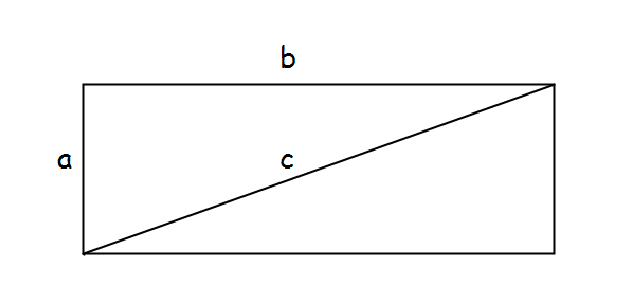
\includegraphics[scale=0.6]{rect.eps}  \hspace*{1cm} 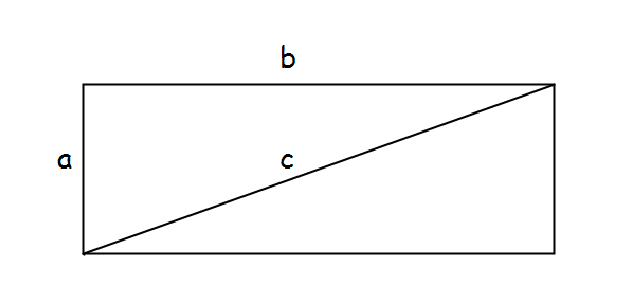
\includegraphics[scale=0.6]{rect.eps} 
\end{center}


- On les assemble ensuite comme indiqué en fabriquant deux carrés ABCD et IJKL.\\

\begin{center}
\includegraphics[scale=1]{thmpyth.eps} 
\end{center}

On considère deux carrés identiques de longueur de côté $a+b$. Chaque figure est constituée de 4 triangles rectangles identiques de longueur a, b et c et d'une partie grise. Le but est de comparer les aires des parties grises des deux figures et d'en déduire une relation entre les mesures a, b et c.\\

\noindent \q Pourquoi les aires des parties grises sont égales ?\\
\q Dans la \textbf{figure A}, quelle est l'expression de l'aire de la partie grise en fonction de a et b.\\
\q Dans la figure B :\\
\hspace*{0.2cm} \qa Déterminer la mesure de l'angle $\widehat{ILK}$.\\
\hspace*{0.2cm} \qa Que peut-on donc dire du quadrilatère IJKL ? \\
\hspace*{0.2cm} \qa Déterminer l'expression de l'aire de la partie grise en fonction de c.\\
\q En fonction des questions précédentes, trouver une relation liant les longueurs a, b et c. 

\noindent \reponse[7]

\newpage

\vspace*{0.3cm}

\textbf{{\large \underline{Démonstration :}}}\\

\initq \q Les aires des surfaces grises dans chaque carré sont égales à l'aire du grand carré moins les aires des quatre triangles identiques.\\ \textbf{Ces aires sont donc égales.}\\

\q Dans la première figure la surface grise est composée de deux carrés, l'un de côté a et l'autre de côté b : \textbf{l'aire grise A est donc égale à $a^{2} + b^{2}$}. \\

\q \qa On sait que les angles $\widehat{DLI}$  et $\widehat{ILK}$ d'une part et les angles $\widehat{ILK}$ et $\widehat{KLC}$ d'autre part sont adjacents.\\
 Par ailleurs, par construction, les points D, L et C sont alignés.\\
 
 On a ainsi :  $\widehat{DLI} + \widehat{ILK} + \widehat{KLC} = \widehat{DLC} = 180 $\degre  \\
 
Or, comme les 4 triangles sont identiques, on déduit que $\widehat{KLC}$ et $\widehat{DLI}$  sont complémentaires. \\

On en déduit que : $\widehat{ILK}= 180 - 90 = 90$\degre.\\

\qa On vient de montrer que le quadrilatère IJKL a un angle droit. Par ailleurs, par construction, les quatre côtés ont la même longueur c. Or, si un losange possède un angle droit alors il en possède 4 et c'est un carré.\\ \textbf{On en déduit ainsi que IJKL est un carré.}\\

\qa On déduit de ce qui précède que dans la deuxième figure la surface grise est un carré de côté c : \textbf{l'aire grise B est donc égale à $c^{2}$}.\\ 

Comme les aires grises des deux figures sont égales, les deux expressions trouvées dans les questions précédentes sont égales. \\

On a donc \fbox{ $a^{2}+b^{2} = c^{2}$}. Ce qui prouve le théorème de Pythagore. \\

\vspace*{2cm}


\underline{\textbf{Pour mercredi 3 ou jeudi 4 octobre :}} Construire sur une grande feuille blanche la démonstration du théorème de Pythagore.

\end{document}
